\documentclass{article}

\usepackage[a4paper, total={16cm, 27cm}]{geometry}
\usepackage{txfonts}
\usepackage{graphicx}
\usepackage{float}
\usepackage[figurename=Figura]{caption}
\usepackage{cite}
\usepackage{url}
\usepackage{hyperref}

\author{Diego Antonio Román Cortés\\Profesor Guía: Rodrigo Andrés Vicencio Poblete}
\date{Departamento de Física, Facultad de Ciencias Físicas y Matemáticas, Universidad de Chile}
\title{Redes interorbitales basadas en moléculas fotónicas}

\begin{document} \maketitle
%Título del proyecto
%Nombre del candidato y del profesor guía o profesores guía

\section{Contexto del proyecto (introducción y descripción del estado del arte)}
	
	Entre los premios Nobel de la última década se encuentran varios que están estrechamente ligados a la óptica: por la generación de pulsos de luz ultra cortos (femtosegundos y luego attosegundos), por experimentos con fotones entrelazados, por la ideación de pinzas ópticas y por la invención de luces LED \cite{nobel}. El estudio del comportamiento de la luz en diversos contextos ha permitido el posterior desarrollo tecnológico con aplicaciones industriales, en medicina, en comunicaciones e incluso militares. Una aplicación cotidiana es la fibra óptica, que actúa como una guía de onda para la luz y actualmente es el principal medio de transmición de Internet en el país \cite{fibra}. 
	
	Numerosos de estos avances se han visto propiciado por la técnica de escritura de guías de onda por láser femtosegundo que ha permitido la fabricación de redes fotónicas de variada índole \cite{femto, bics, lieb1, lieb2, artificialFB, FBdynamics}. Su importancia radica no sólo en emular situaciones de la física del sólido, sino que también en el estudio de fenómenos ópticos como la no-linealidad tipo Kerr, la posibilidad de propagar luz cuántica o su compatinilidad con la transmición en la industria de telecomunicaciones \cite{discretesolitons, qed, squeezed, topoquantum, telecom}.
	
	En particular, el acoplamiento interorbital SP ha permitido el estudio de redes que presentan flujo magnético efectivo $\Phi = \pi$ el cual permite el transporte controlado de la luz \cite{interorbital, OAMCaging, ABCaging}. Se ha reportado la propagación de luz con momentum angular orbital (OAM) sólo mediante de redes fotónicas que presevan simetría $C_3$ \cite{OAMWG, vortex}. Sin embargo, el acoplamiento entre modos OAM permitiría la generación de flujos magnéticos distintos de $0$ o $\pi$ y por tanto una direccionalidad dependiente de la circulación propagante \cite{vortextrim, topoOAM}.
\section{Objetivos de la tesis}
\begin{enumerate}
	\item Utilizar moléculas fotónicas como base para fabricar y estudiar redes interorbitales.
	\item Entender el comportamiento de los modos guiados en moléculas fotónicas y su interacción en el régimen de acoplamiento débil.
\end{enumerate}
\section{Metodología}

Desde las ecuaciones de Maxwell en un medio dieléctrico no magnético sin cargas ni corrientes libres es posible escribir la siguiente ecuación para la envolvente lenta del campo eléctrico $\textbf{E}(\textbf{r}) = \textbf{E}_1(\textbf{r}) e^{-i \textbf{k}_1 \cdot \textbf{r}}$.

\begin{equation}
	(\nabla-i\textbf{k}_1)\times(\nabla-i\textbf{k}_1)\times \textbf{E}_1 = k^2 \textbf{E}_1,
	 \label{eqn:maxwell}
\end{equation}
con $k \equiv k_0 n$.
La ecuación (\ref{eqn:maxwell}) es resuelta por el software comercial COMSOL \textit{Multiphysics} mediante elementos finitos y será una de las herramientas a usar en esta tesis. Por otro lado, utilizando la aproximación paraxial es posible simplificar la ecuación (\ref{eqn:maxwell}) y llegar a la implementación de los \textit{Beam Propagation Methods} usados ampliamente en el área \cite{bics, interorbital, OAMCaging, vortex, bpm}.
\begin{equation}
	-i\lambdabar\frac{\partial}{\partial z}\psi(x,y,z) = \left(\frac{\lambdabar^2\nabla_\perp^2}{2n_0} + \Delta n(x,y)\right) \psi (x,y,z) \label{eqn:paraxial}
\end{equation}

Aplicando teoría acoplada de modos a la ecuación (\ref{eqn:paraxial}) para describir de forma discreta una red fotónica, es posible derivar las ecuaciones discretas tipo Schrödinger para la envolvente normalizada del campo eléctrico \cite{discretesolitons}:
\begin{equation}
	-i\frac{\partial u_{\vec{n}} }{\partial z} = \beta_{\vec{n}}u_{\vec{n}} + \sum_{\vec{m}\neq\vec{n}} C_{\vec{n},\vec{m}}u_{\vec{m}} \label{eqn:CMT}
\end{equation}

Para la fabricación de guías de onda se utiliza un láser femtosegundo pulsado de 1064 nm enfocado en un vidrio de borosilicato en movimiento gracias a una plataforma XYZ motorizada.

\begin{figure}[H]
	\centering
	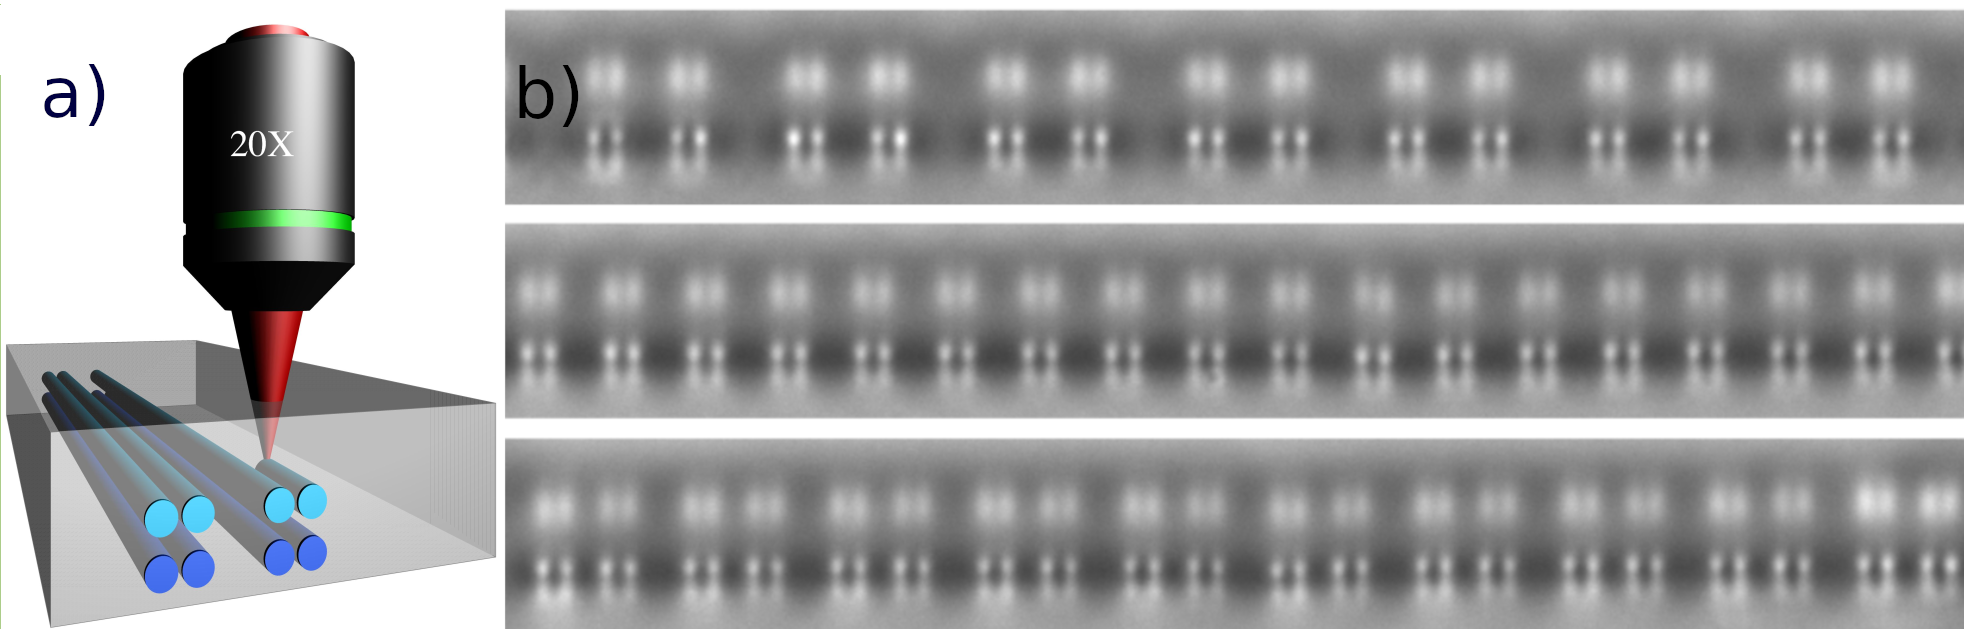
\includegraphics[width=0.9\linewidth]{./media/femtosetup.png}
	\caption{a) Montaje de fabricación de guías de onda mediante el enfoque de láser femtosegundo. b)      Imagen microscópica de la cara salida iluminada con luz blanca. \label{fig:SLM}}
\end{figure}


La excitación de redes fotónicas interorbitales hace necesario el uso de condiciones iniciales no triviales. Para ello se implementó una técnica de modulación espacial de luz que permite modular tanto la amplitud como la fase de el haz tipo gaussiano proveniente del láser \cite{slm}.

\begin{figure}[H]
	\centering
	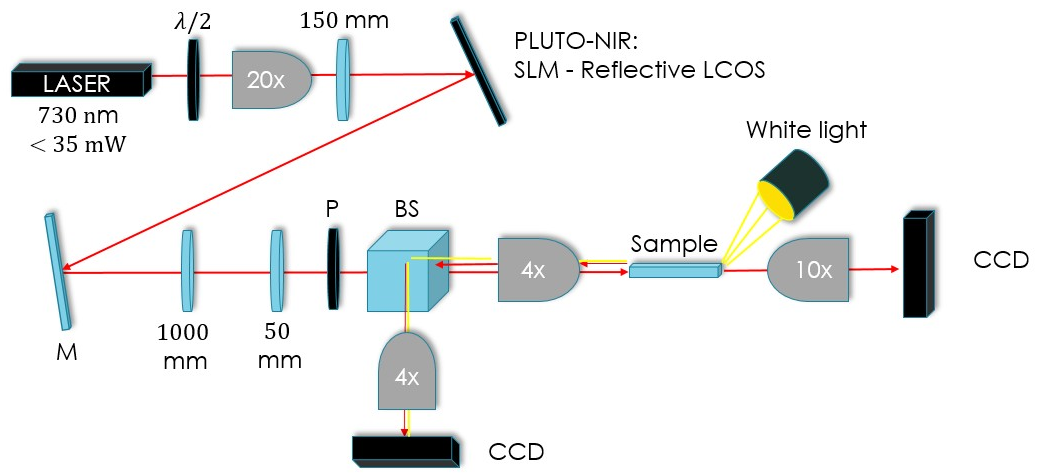
\includegraphics[width=0.9\linewidth]{./media/SLMsetup.png}
	\caption{Montaje de excitación de guías de onda con condiciones iniciales moduladas en amplitud y fase.\label{fig:femtosetup}}
\end{figure}

\section{Trabajo adelantado (si lo hubiera)}

Durante el curso de Seminario de Investigación I (Primavera 2022) se hizo un barrido de parámetros de fabricación de guías de onda, en particular de potencia de escritura y separación entre guías, logrando la inversión de elipticidad el sintonizado de las constantes de propagación del modo fundamental $S$ de la molécula de excitación y el modo excitado $P_x$ de la molécula de acoplamiento.


\begin{figure}[H]
	\centering
	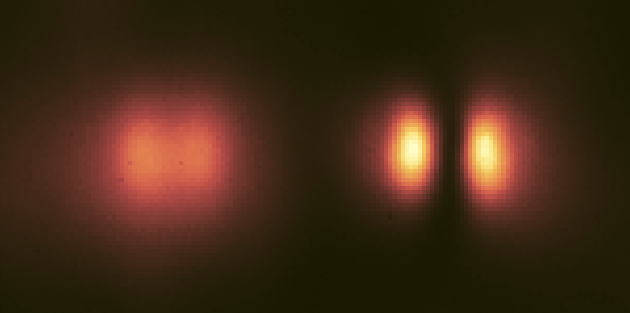
\includegraphics[width=0.5\linewidth]{./media/SPinteraction.png}
	\caption{Interacción interorbital en moléculas fotónicas a 25 $\mu$m de sepración y 13 mm de propagación. Se inyecta luz láser en la molécula S ubicada a la izquierda.}
\end{figure}

Durante el curso de Seminario de Investigación II (Otoño 2023) se implementó el montaje de modulación esquematizado en la Figura \ref{fig:SLM}. Con ello fue posible la excitación de un dipolo horizontal:

\begin{figure}[H]
	\centering
	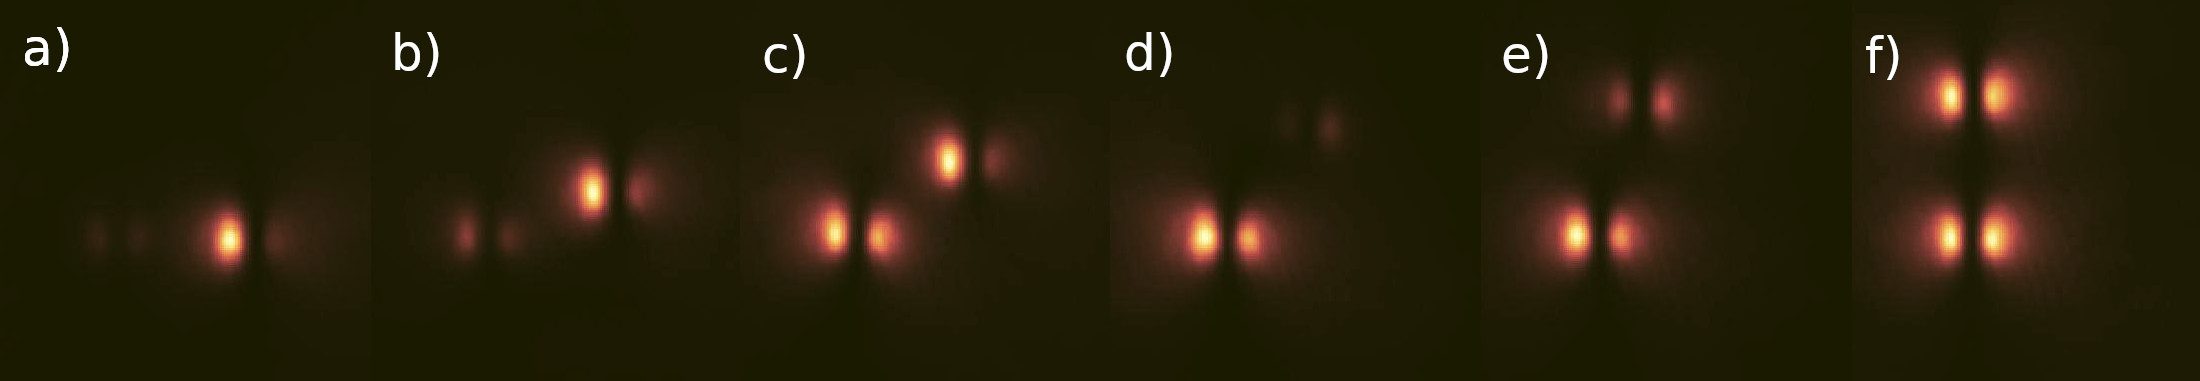
\includegraphics[width=1.0\linewidth]{./media/dipoles.jpg}
	\caption{a)-f) Barrido en ángulo de dímeros dipolares a una distancia de separación de 25 $\mu$m propagando en una distancia de 25 mm en la dirección perpencicular al plano. La inyección se realiza en la molécula inferior izquierda con un modo Hermite-Gauss TEM$_{10}$. En d) se pasa por el ángulo mágico que hace nula la interacción dipolar.}
\end{figure}

Se está trabajando en la excitación de un OAM con $l = \pm 1$ usando la técnica de modulación espacial de la Figura \ref{fig:SLM}:

\begin{figure}[H]
	\centering
	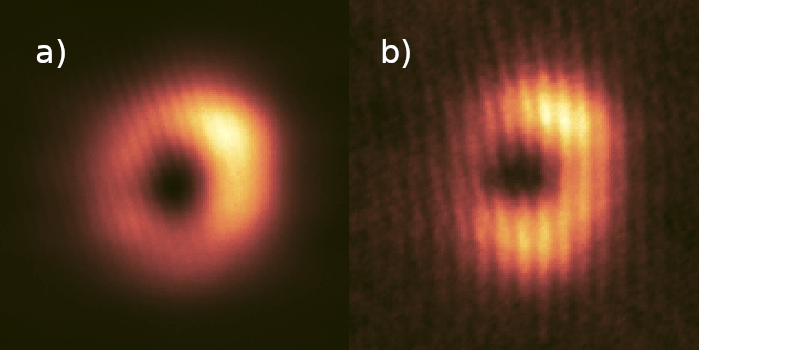
\includegraphics[width=0.7\linewidth]{./media/vortex.png}
	\caption{a) Intensidad de un OAM propagado en una molécula fotónica. b) Interferograma que captura el cambio de fase esperado.}
\end{figure} 

\section{Plan de trabajo o carta Gantt}


% citations
\renewcommand\refname{Referencias}
\bibliographystyle{ieeetr}
\bibliography{citations}

\end{document}
